
% this file is called up by thesis.tex
% content in this file will be fed into the main document

%: ----------------------- introduction file header -----------------------
\chapter{Semantic Web Background Technologies} \label{cha:background}

% the code below specifies where the figures are stored
\ifpdf
    \graphicspath{{2_background/figures/PNG/}{2_background/figures/PDF/}{2_background/figures/}}
\else
    \graphicspath{{2_background/figures/EPS/}{2_background/figures/}}
\fi

% ----------------------------------------------------------------------
%: ------------------------------- content ----------------------------- 
% ----------------------------------------------------------------------

The main contributions of this thesis are methods for the automatic generation of
user-customizable media galleries for the visual and audial summarization of events.
To provide context for the approaches proposed in the later parts of the thesis,
we start with an introduction of related Semantic Web background technologies.
The current \autoref{cha:background} covers the Semantic Web, Linked Data,
and the Resource Description Framework (RDF).
The following \autoref{cha:social-networks} will cover social networks
by first providing a~definition and classification of social networks,
and then introducing popular social networks and some of their core features.

\section{Semantic Web}
The lexical database WordNet~\cite{Fellbaum1998} by the Cognitive Science Laboratory
of Princeton University defines\footnote{\url{http://wordnetweb.princeton.edu/perl/webwn?s=semantic}}
the term \emph{semantic} as \emph{of or relating to meaning or the study of meaning}.
The same source defines\footnote{\url{http://wordnetweb.princeton.edu/perl/webwn?s=world+wide+web}}
the term \emph{Web}, which is a~common form for the complete term \emph{World Wide Web} (or just \emph{WWW}) as
\emph{computer network consisting of a~collection of internet sites that offer text and graphics and
sound and animation resources through the hypertext transfer protocol}.
Finally WordNet defines\footnote{\url{http://wordnetweb.princeton.edu/perl/webwn?s=meaning}}
the term \emph{meaning} as \emph{the message that is intended or expressed or signified}, or
\emph{the idea that is intended}.

The combined term \emph{Semantic Web} has been coined by Sir Tim Berners-Lee,
the inventor of the World Wide Web and Director of the World Wide Web Consortium,
in a~May 2001 article co-published with James Hendler and Ora Lassila
in the Scientific American~\cite{BernersLee2001}.
Therein, the authors write: 

\begin{quotation}
``The Semantic Web will bring structure to the meaningful content of Web pages,
creating an environment where software agents roaming from page to page
can readily carry out sophisticated tasks for users. [\ldots]
The Semantic Web is not a~separate Web but an extension of the current one,
in which information is given well-defined meaning, better enabling computers and people
to work in cooperation.
The first steps in weaving the Semantic Web into the structure of the existing Web
are already under way.
In the near future, these developments will usher in significant new functionality
as machines become much better able to process and \emph{understand} the data
that they merely display at present.''
\end{quotation}

We are currently experiencing a~fundamental shift from the World Wide Web (WWW) to the Semantic Web,
a~shift from moving bits to moving bits with a~meaning.
This can have a~huge impact, which might not be as drastic as Tim Berners-Lee describes
in his Scientific American article, but which might introduce many small improvements,
like more accurate search results, or more intelligent price comparison services etc.
\autoref{fig:fundamental-shift} illustrates this idea.

\begin{figure}[htbp!]
\begin{center}
  \subfloat[Bits without meaning.]{\label{fig:fundamental-shift-1}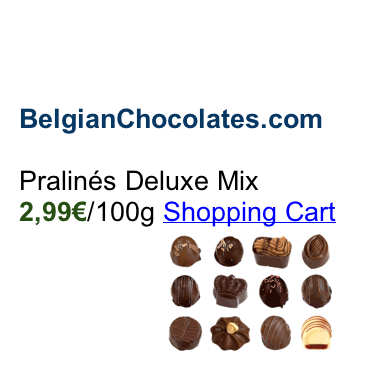
\includegraphics[width=0.3\textwidth]{fundamental-shift-1.png}}                
  \subfloat[Bits with a~meaning.]{\label{fig:fundamental-shift-2}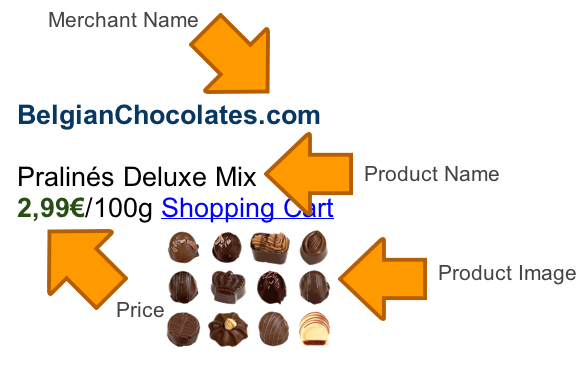
\includegraphics[width=0.468\textwidth]{fundamental-shift-2.png}}
  \caption{Fundamental shift from moving bits to moving bits with a~meaning.}
  \label{fig:fundamental-shift}  
\end{center}    
\end{figure}

\subsection{The Non-Semantic Web} \label{sec:non-semantic-web}
To differentiate the Semantic Web from the non-semantic Web, it helps to step back one step and
see why the non-semantic Web is not semantic.
The Web is a~system of interlinked hypertext documents accessed through the Internet.
These documents are typically marked up in HTML, a~language that defines a~syntax
understandable to user agents like Web browsers, however,
not one that provides meaning beyond the level of text layout.
This means that an HTML snippet like
\begin{verbatim}
<h1>The Catcher in the Rye</h1>
<h2>J. D. Salinger</h2>
\end{verbatim}
reveals that \emph{The Catcher in the Rye} is a~level one header element and
that \emph{J. D. Salinger} a~level two header element,
but to a~machine it is not evident that the prior is the title of a~book,
and that the latter is (i), an author, and (ii), the author of \emph{The Catcher in the Rye}.

\subsection{Structured Data on the Web}
A very first step to add semantics to the Web is using tabular data.
\autoref{tab:sample-table-structured-data} shows an example for such tabular data.
To human beings (interested in sports), the meaning of the columns is clear:

\begin{table}[b]
 \begin{center}
  \begin{tabular}{l*{6}{c}r}
Team              & P & W & D & L & F  & A & Pts \\
\hline
Manchester United & 6 & 4 & 0 & 2 & 10 & 5 & 12  \\
Celtic            & 6 & 3 & 0 & 3 &  8 & 9 &  9  \\
Benfica           & 6 & 2 & 1 & 3 &  7 & 8 &  7  \\
FC Copenhagen     & 6 & 2 & 1 & 2 &  5 & 8 &  7  \\
  \end{tabular}
\caption{Sample table with structured data for sports results.}
\label{tab:sample-table-structured-data}
 \end{center}
\end{table}

\begin{itemize}
\item P = matches \textbf{P}layed
\item W = \textbf{W}on 
\item D = \textbf{D}rew
\item L = \textbf{L}oss
\item F = Goals \textbf{F}or
\item A = Goals \textbf{A}gainst
\item Pts = \textbf{P}oin\textbf{ts}
\end{itemize}

The problem, however, is for machines to understand the structure of the table.
Let us imagine one wanted to automate the task of retrieving sports results.
While it is a~relatively straightforward job to implement a~scraper bot that
searches for column titles like ``P'', ``W'', ``D'' etc.,
it would require the same work over and over again for different languages
(for example German for: ``Sp.'', ``g.'', ``u.'', ``v.'', ``Tore'', ``Pkte.'').
The German-speaking reader might have noticed that the exemplary German system listed here
does not differentiate between \emph{goals for} and \emph{goals against}, but only has a~list of \emph{Goals}.
Tiny differences like this make the scraping approach so brittle.
If data providers were to use unique column identifiers like URIs, the problem would be mostly gone.
In the concrete example, rather than using ``D'' or ``u.'', which both mean that the result was a~tie,
the machine-readable column name could be identified by the URI
\url{http://dbpedia.org/page/Tie_%28draw%29}.
In the next Section we therefore introduce the structured knowledge base DBpedia.

\subsection{The Structured Knowledge Base DBpedia}
An often reoccurring (however not binding) pattern in the Semantic Web world
is the use of DBpedia~\cite{Auer2007} URIs as a~hub for identifying concepts by URIs.
DBpedia is a~Semantic Web knowledge base with the objective of
automatically extracting structured data from the human-generated information from
the online encyclopedia Wikipedia~\footnote{\url{http://en.wikipedia.org/wiki/Main_Page}}.
This structured information is then made available on the World Wide Web in many variations,
for example as JSON~\cite{Crockford2006}, HTML~\cite{LeHors1999}, XML~\cite{Bray1998},
and many RDF~\cite{Klyne2004} serializations.
DBpedia allows for querying relationships and properties associated with Wikipedia resources,
including links to other related datasets.
As outlined before, the concept of a~tie draw in the sense of sports
could thus be uniquely identified by the DBpedia URI \url{http://dbpedia.org/page/Tie_%28draw%29},
free of all ambiguity.
Similar knowledge bases are among others Freebase~\cite{Markoff2007},
YAGO~\cite{Suchanek2007}, or Cyc~\cite{Wilkins1997}.

\subsection{Semantics in HTML Version 4 and 5}
As outlined in \autoref{sec:non-semantic-web}, HTML versions 4~\cite{LeHors1999} and 5~\cite{Hickson2011}
contain a~basic level of semantics.
The main focus, however, is on the separation of semantics from presentation.
For example the \texttt{<b>} and the \texttt{<strong>} tags both have the same visual effect:
they make the node value appear in a~bold face \textbf{like so}.
Visually, there is no way to differentiate between the two, however,
semantically the difference exists and is well-defined:
\texttt{<strong>} should be used when one wants to give special emphasis on something,
screenreaders will typically read out such text with a~more emphasized voice.
In contrast \texttt{<b>} should be used if only visually one wants to create a~bold face look.
In the following, we present a~list of semantic HTML tags and attributes and their meaning.
The list is inspired by an
extension\footnote{\url{https://addons.mozilla.org/en-us/firefox/addon/semantic-checker/}}
for the Web browser Firefox.

\paragraph{Semantic HTML4 Elements}
\begin{itemize}
\item \texttt{abbr} specifies an abbreviation, \texttt{acronym} specifies an acronym.
\item \texttt{h1-h6} specify level 1–6 headers, \texttt{caption} specifies a~caption for a~table.
\item \texttt{blockquote} specifies a~block-level quotation
(a source in form of a~URI may be specified via the \texttt{@cite} attribute),
\texttt{cite} specifies a~citation.
\item \texttt{dl} specifies a~definition list, \texttt{dt} specifies a~definition term in a~definition list,
\texttt{dd} specifies the definition of a~term in a~definition list.
\item \texttt{em} specifies an emphasis, \texttt{strong} specifies a~strong emphasis.
\item \texttt{code} specifies a~code snippet, \texttt{dfn} specifies an inline definition of a~single term,
\texttt{address} specifies contact information for the document author,
\texttt{legend} specifies a~legend for \texttt{fieldset} containers for adding structure to forms,
\texttt{samp} specifies sample output from a~script or program.
\end{itemize}

\paragraph{Semantic HTML5 Elements}
\begin{itemize}
\item \texttt{article} specifies an independent item section of content,
\texttt{aside} specifies a~section of a~page that consists of content that is tangentially related
to the content around the \texttt{aside} element, and which could be considered separate from that content,
\texttt{header} specifies a~group of introductory or navigational aids,
\texttt{footer} specifies a~footer for its nearest ancestor sectioning content or sectioning root element,
\texttt{nav} specifies a~section with navigation links.
\item \texttt{figure} specifies some flow content,
\texttt{mark} specifies a~run of text in one document marked or highlighted for reference purposes
due to its relevance in another context, \texttt{meter} specifies a~scalar measurement within
a~known range, or a~fractional value.
\item \texttt{audio} specifies a~sound or an audio stream, \texttt{video} specifies a~video or movie.
\item \texttt{progress} specifies the completion progress of a~task,
\texttt{time} specifies either a~time on a~24 hour clock,
or a~precise date in the calendar (optionally with a~time and a~time-zone offset),
\texttt{command} specifies a~command that the user can invoke.
\item \texttt{details} specifies a~disclosure widget
from which the user can obtain additional information or controls,
\texttt{datalist} specifies the list that represent predefined options for input elements.
\item \texttt{keygen} specifies a~key pair generator control,
\texttt{output} specifies the result of a~calculation,
\texttt{ruby} allows one or more spans of phrasing content to be marked with ruby annotations.
\end{itemize}

\paragraph{HTML5 Input Attributes}
\begin{itemize}
\item \texttt{datetime} specifies a~control for setting the element’s value
to a~string representing a~global date and time (with timezone information).
\item \texttt{datetime-local} specifies a~control for setting the element’s value
to a~string representing a~local date and time (with no timezone information).
\item \texttt{date} specifies a~control for setting the element’s value
to a~string representing a~date, \texttt{month} specifies a~control
for setting the element’s value to a~string
representing a~month, \texttt{week} specifies a~control for setting the element’s value
to a~string representing a~week.
\item \texttt{time} specifies a~control for setting the element’s value
to a~string representing a~time (with no timezone information.
\item \texttt{number} specifies a~control for setting the element’s value
to a~string representing a~number.
\item \texttt{range}  represents an imprecise control for setting the element’s value
to a~string representing a~number.
\item \texttt{email} specifies a~control for editing a~list of email addresses
given in the element’s value.
\item \texttt{url} specifies a~control for editing an absolute URL
given in the element’s value.
\item \texttt{search} specifies a~one-line plain-text edit control
for entering one or more search terms.
\item \texttt{color} specifies a~color-well control for setting the element’s value
to a~string representing a~simple color.
\end{itemize}

\subsection{Structured Data Beyond Pure HTML}
In this Subsection, we describe how structured data can be included in HTML documents
by either overloading existing HTML attributes, or by adding new HTML attributes.

\subsubsection{Microformats}
Microformats~\cite{Celik2006} are a~set of open data mark-up formats developed
and defined by the Microformats community\footnote{\url{http://microformats.org/discuss}}.
Microformats are not an official standard, but rather a~widely adopted grass-roots-driven movement
with origins in the blogging scene.
It is to be noted that Microformats do not require a~new language,
but reuse building blocks from widely adopted standards such as the \texttt{@class},
\texttt{@rel}, and \texttt{@title} attributes in HTML.
Their main design goal is to focus first on humans, then on machines.
A concrete example of Microformat mark-up in HTML can be seen in \autoref{code:microformats}.
There are currently nine stable
Microformats\footnote{\url{http://microformats.org/wiki/Main_Page\#Specifications}},
as listed below:

\begin{itemize}
\item \texttt{hCalendar} is a~distributed calendaring and events format, using a~1:1 representation of the standard \texttt{iCalendar} format (RFC2445,~\cite{Dawson-1-1998}).
\item \texttt{hCard} is a~format for representing people, companies, organizations, and places, using a~1:1 representation of the standard \texttt{vCard} format (RFC2426,~\cite{Dawson-2-1998}).
\item \texttt{rel-license} is a~format for indicating content licenses, which is embeddable in HTML~\cite{LeHors1999} or XHTML~\cite{Pemberton2000}, Atom~\cite{Nottingham2005}, RSS~\cite{Cadenhead2006}, and arbitrary XML~\cite{Bray1998}.
\item \texttt{rel-nofollow} is a~format for hyperlinks indicating that the destination of that hyperlink should not be afforded any additional weight or ranking by user agents such as search engines, which perform link analysis upon Web pages.
\item \texttt{rel-tag} format for hyperlinks indicating that the destination of that hyperlink is an author-designated keyword for the current page.
\item \texttt{VoteLinks} is a~format for adding the idea of agreement, abstention or indifference, and disagreement to hyperlinks.
\item \texttt{XFN} is a~format for representing human relationships using hyperlinks, which enables Web authors to indicate their relationships to people.
\item \texttt{XMDP} is a~format for defining metadata profile documents (XHTML Meta Data Profile), which enables Web authors to well-define custom meta tags.
\item \texttt{XOXO} is a~format for defining a~new XHTML document type for subsetting and extending XHTML, which serves as the basis for XHTML-friendly outlines for processing by XML engines, and for easy interactive rendering by browsers.
\end{itemize}

\begin{lstlisting}[caption={[Sample code snippet with embedded hCard Microformat mark-up.]{Sample code snippet with embedded \texttt{hCard} Microformat mark-up. Source: \url{http://microformats.org/wiki/hcard}}},label={code:microformats}]
<div class="vcard">
  <a class="fn org url" href="http://www.commerce.net/">CommerceNet</a>
  <div class="adr">
    <span class="type">Work</span>:
    <div class="street-address">169 University Avenue</div>
    <span class="locality">Palo Alto</span>,  
    <abbr class="region" title="California">CA</abbr>&nbsp;&nbsp;
    <span class="postal-code">94301</span>
    <div class="country-name">USA</div>
  </div>
  <div class="tel">
   <span class="type">Work</span> +1-650-289-4040
  </div>
  <div class="tel">
    <span class="type">Fax</span> +1-650-289-4041
  </div>
  <div>Email: 
   <span class="email">info@commerce.net</span>
  </div>
</div>
\end{lstlisting}

\subsubsection{Microdata}
Microdata~\cite{Hickson2010} defines a~way to annotate content (or items) with specific machine-readable labels,
for example to allow scripts to provide services that are customized to a~website.
Microdata allows nested groups of name-value pairs to be added to documents,
in parallel with the existing content.
The Microdata specification introduces a~set of new attributes to HTML:

\begin{itemize}
\item \texttt{itemscope}: creates an item (or thing) and indicates that descendants of this element contain information about it. This attribute precedes the \texttt{itemtype} attribute in the HTML element's tag.
\item \texttt{itemtype}: a~valid URL of a~vocabulary that describes the item and its properties context.
\item \texttt{itemid}: indicates a~unique identifier of the item in the vocabulary.
\item \texttt{itemprop}: indicates that its containing tag holds the value of the specified item property. The properties name and value context are described by the items vocabulary. Properties values usually consist of string values, but can also use URLs using the \texttt{a} element and its \texttt{href} attribute, the \texttt{img} element and its \texttt{src} attribute, or other elements that link to or embed external resources.
\item \texttt{itemref}: properties that are not descendants of the element with the \texttt{itemscope} attribute can be associated with the item using this attribute. Provides a~list of elements to web crawlers to find additional property values of the item elsewhere in the document.
\end{itemize}

An example of Microdata in HTML can be seen in Figure~\ref{code:microdata}

\begin{lstlisting}[caption={[Sample code snippet with Microdata mark-up.]{Sample code snippet with Microdata mark-up. Source: \url{http://www.w3.org/TR/microdata/}}},label={code:microdata}]
<div itemscope>
  <p>My name is <span itemprop="name">Neil</span>.</p>
  <p>
    My band is called
    <span itemprop="band">Four Parts Water</span>.
  </p>
  <p>I am <span itemprop="nationality">British</span>.</p>
</div>
\end{lstlisting}

\section{Resource Description Framework (RDF)} \label{sec:rdf}
The Resource Description Framework (RDF)~\cite{Klyne2004} defines
a~set of W3C standards for the formal description of resources that are identified by URIs.
RDF is a~core component of the Semantic Web.
Initially it was designed to describe metadata on the World Wide Web (WWW) such as authors,
copyrights, etc. of documents, however, using a~definition of the term \emph{resource}
beyond the WWW context, RDF is now also used to describe metadata of any URI-identifiable entity.

\subsection{Triples as a~Data Structure}
As outlined before, one of the main purposes of the Semantic Web is to give information
a~well-defined meaning.
Using an example from Berners-Lee’s article~\cite{BernersLee2001},
meaning can be to differentiate between the concepts of a~shipping and a~billing address,
or the concept of an address in the sense of delivering a~formal spoken communication to an audience.
In order to assure the differences in meaning,
things are identified by a~Unique Resource Identifier (URI).
The majority of the data processed by machines can be described by elementary sentences like
\emph{A cat is a~mammal}, \emph{Thomas Steiner is author of this document}, or
\emph{Prince William is married to Kate Middleton}.
Each of these sentences has a~subject (\emph{A cat}), a~predicate (\emph{is a}),
and an object (\emph{mammal}).
Every subject, predicate, and object can be identified by a~URI.
This concept turns out to be very powerful, as it allows to express the same concept,
represented by a~URI (like for example mammal by \url{http://dbpedia.org/resource/Mammal})
with different terms in different languages (like for example Säugetier, mammal, or nisäkkäät). 
Everyone can extend the set of concepts, simply by creating a~URI on the Web.
This form of knowledge representation is used by the Resource Description Framework, or short RDF.

\subsection{Important RDF Serialization Syntaxes}
The knowledge represented in the RDF triple data structure needs to be serialized
in order to be stored or transmitted over the Internet.
Several serialization formats exist, each of which has its particular advantages
and disadvantages, mostly around readability for human beings and parsability for machines.
Most people prefer the Turtle~\cite{Prudhommeaux2011} format for its readability,
whereas for machines N-Triples~\cite{Grant2004} is the easiest to parse.

\subsubsection{RDF Sample Graph}
In the following, we will illustrate the various RDF serialization formats
with an RDF sample graph, which is introduced here.
It contains data about a~FOAF~\cite{Brickley2010} person named \emph{John X. Foobar},
and an email address with an SHA1 checksum of \emph{cef817456278b70cee8e5a1611539\-ef9d928810e}.
The actual email address is obscured to avoid spam emails.
\autoref{fig:sample-rdf-graph} shows the graphical representation of this sample graph.

\begin{figure}[htbp!]
\begin{center}
 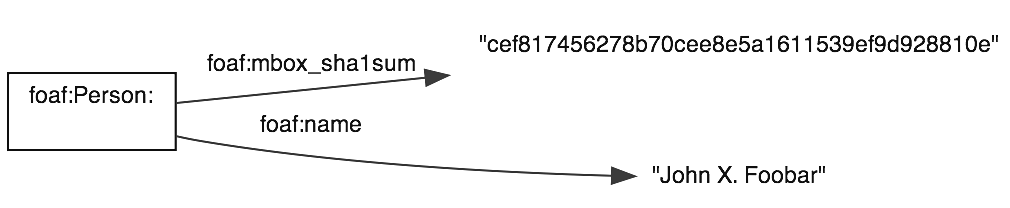
\includegraphics[width=\linewidth]{sample-rdf-graph.png} 
 \caption{A sample RDF graph visualized.}
 \label{fig:sample-rdf-graph}
 \end{center}  
\end{figure}

\subsubsection{The Notation3 Syntax} \label{sec:notation3}
Notation3~\cite{BernersLee2011} was introduced by Tim Berners-Lee.
Notation3 has some features that go beyond the pure expressiveness of RDF, like rules.
Its media type is \texttt{text/n3;\-charset=utf-8},
the recommended file extension is \texttt{.n3}, the encoding is always UTF-8.
\autoref{code:notation3-syntax} shows the previously introduced sample graph serialized in Notation3.

\begin{lstlisting}[caption={A sample graph in Notation3 syntax.},label={code:notation3-syntax}]
@prefix foaf: <http://xmlns.com/foaf/0.1/> .

_:node15urahancx74223 a foaf:Person ;
  foaf:name "John X. Foobar" ;
  foaf:mbox_sha1sum "cef817456278b70cee8e5a1611539ef9d928810e" .
\end{lstlisting}

\subsubsection{The Turtle Syntax} \label{sec:turtle}
Turtle~\cite{Prudhommeaux2011} was developed by Dave Beckett and Tim Berners-Lee
It is a~superset of N-Triples (see \autoref{sec:n-triples}) and
a subset of Notation3 (see \autoref{sec:notation3}).
It has reached a~\emph{de facto} standard status.
Its media type is \texttt{text/turtle}
(the sometimes still observable media type \texttt{application/x-turtle} is deprecated),
the recommended file extension is \texttt{.ttl}, the encoding is UTF-8.
\autoref{code:turtle-syntax} shows the previously introduced sample graph serialized in Turtle.

\begin{lstlisting}[caption={A sample graph in Turtle syntax.},label={code:turtle-syntax}]
@prefix foaf: <http://xmlns.com/foaf/0.1/> .

_:node15urahancx74223 a foaf:Person ;
  foaf:name "John X. Foobar" ;
  foaf:mbox_sha1sum "cef817456278b70cee8e5a1611539ef9d928810e" .
\end{lstlisting}

\subsubsection{The N-Triples Syntax} \label{sec:n-triples}
The N-Triples~\cite{Grant2004} syntax was primarily developed by Dave Beckett and Art Barstow.
N-Triples is a~subset of Turtle (see \autoref{sec:turtle}),
which in turn is a~subset of Notation3 (see \autoref{sec:notation3}).
There are very few variations to express a~graph in N-Triples,
which makes it an ideal syntax for testing purposes, however,
as it is missing some shortcuts of Turtle, it is quite verbose.
Its media type is \texttt{text/plain}, the recommended file extension is \texttt{.nt},
and the encoding is 7-bit US-ASCII.
\autoref{code:ntriples-syntax} shows the previously introduced sample graph serialized in N-Triples.

\begin{lstlisting}[caption={A sample graph in N-Triples syntax.},label={code:ntriples-syntax}]
_:1 <http://www.w3.org/1999/02/22-rdf-syntax-ns#type>
    <http://xmlns.com/foaf/0.1/Person> .
_:1 <http://xmlns.com/foaf/0.1/name>
    "John X. Foobar" .
_:1 <http://xmlns.com/foaf/0.1/mbox_sha1sum>
    "cef817456278b70cee8e5a1611539ef9d928810e" .
\end{lstlisting}

\subsubsection{The RDF/XML Syntax}
RDF/XML~\cite{Beckett2004} was introduced by the W3C as the first RDF serialization syntax.
Albeit more human-friendly serialization formats such as Turtle are gaining more and more traction,
RDF/XML is still very wide-spread.
Its media type is \texttt{application/rdf+xml}, the recommended file extension is \texttt{.rdf},
the encoding is UTF-8.
\autoref{code:rdfxml-syntax} shows the previously introduced sample graph serialized in RDF/XML.

\begin{lstlisting}[caption={A sample graph in RDF/XML syntax.},label={code:rdfxml-syntax}]
<?xml version="1.0" encoding="UTF-8"?>
<rdf:RDF
    xmlns:foaf="http://xmlns.com/foaf/0.1/"
    xmlns:rdf="http://www.w3.org/1999/02/22-rdf-syntax-ns#">
  <rdf:Description rdf:nodeID="node15urahancx74224">
    <rdf:type rdf:resource="http://xmlns.com/foaf/0.1/Person"/>
    <foaf:name>John X. Foobar</foaf:name>
    <foaf:mbox_sha1sum>
      cef817456278b70cee8e5a1611539ef9d928810e
    </foaf:mbox_sha1sum>
  </rdf:Description>
</rdf:RDF>
\end{lstlisting}

\subsubsection{The RDFa Syntax}
RDFa has a~special role in that it is a~specification for attributes to express structured data
in XHTML~\cite{Adida2008} (but also standard HTML).
It uses the rendered hypertext content of XHTML for the RDFa markup,
so that data publishers can use the same document for human- and machine-readable content.
There is also a~specification for RDFa 1.1 in HTML4 and HTML5~\cite{Sporny2011}.
The contained RDF triples can be extracted with distillers,
in consequence RDFa can be considered as another serialization syntax for RDF,
with the same expressive power as RDF/XML or Turtle.
Its media type is \texttt{application/xhtml+xml}, the recommended file extension is \texttt{.html}.
RDFa shares some design goals with Microformats~\cite{Celik2006}
Where Microformats specify both a~syntax for embedding structured data into HTML
\emph{and} a~vocabulary of specific terms for each Microformat,
RDFa in contrast \emph{only} specifies a~syntax.
RDFa relies on independent external specifications of vocabularies.
The essence of RDFa is a~set of attributes that contain metadata about things,
and that can be embedded in mark-up languages, for example in XHTML or HTML.
The concrete attributes are:

\begin{itemize}
\item \texttt{about} and \texttt{src}: a~URI or CURIE (compact URI expressions) specifying the resource the metadata is about.
\item \texttt{rel}: specifying a~relationship with another resource.
\item \texttt{href} and \texttt{resource}: specifying the partner resource.
\item \texttt{property}: specifying a~property for the content of an element.
\item \texttt{content}: optional attribute that overrides the content of the element when using the property attribute.
\item \texttt{datatype}: optional attribute that specifies the datatype of text specified for use with the property attribute.
\item \texttt{typeof}: optional attribute that specifies the RDF type(s) of the subject (the resource that the metadata is about).
\end{itemize}

\autoref{code:rdfa-syntax} shows the previously introduced sample graph serialized in RDFa.

\begin{lstlisting}[caption={A sample graph in RDFa syntax.},label={code:rdfa-syntax}]
<div about="_:1" typeof="http://xmlns.com/foaf/0.1/Person">           
  <span property="http://xmlns.com/foaf/0.1/mbox_sha1sum">
    cef817456278b70cee8e5a1611539ef9d928810e
  </span> 
  <span property="http://xmlns.com/foaf/0.1/name">
    John X. Foobar
  </span>
</div> 
\end{lstlisting}

\section{SPARQL -- Semantic Web Query Language}
SPARQL is a~recursive acronym that stands for SPARQL Protocol and RDF Query Language.
The SPARQL specification~\cite{Prudhommeaux2008} defines the syntax and semantics
of the SPARQL query language for RDF.
RDF~\cite{Klyne2004} is a~directed, labeled graph data format for representing information in the Web.
SPARQL can be used to express queries across diverse data sources,
whether the data is stored natively as RDF, or viewed as RDF via middleware.
SPARQL allows for querying required and optional graph patterns
along with their conjunctions and disjunctions.
SPARQL also supports extensible value testing and constraining queries by source RDF graph.
The results of SPARQL queries can be results sets or RDF graphs.
SPARQL became an official World Wide Web Consortium (W3C) Recommendation in the year 2008.
It was standardized by the RDF Data Access Working Group (DAWG).

\subsection{The Vision of the Web as a~Giant, Single Database}
The Web as we know it today is a~\emph{network of documents} interconnected by hyperlinks
that everyone can participate in by placing links to existing documents.
The vision of the Semantic Web, however, is a~\emph{network of facts} about entities,
interconnected in form of graphs of data.
Where the Web of today is a~graph of documents, the Semantic Web is envisioned to be a~huge global graph,
formed by many, many individual graphs.
If one party publishes facts about an entity, and a~different party publishes different facts
about the same entity, then the overall knowledge about that entity is represented in a~decentralized way,
accessible to all, and open for everyone to enrich.
This obviously requires strong globally unique identifiers,
or at least ways to map one identifier to another.

Given the (visionary) huge global graph, a~SPARQL query like the one in \autoref{code:sparql}
could be used to get results from the graph,
like the email addresses of every person in the world.

\begin{lstlisting}[caption={[SPARQL query returning the names and email addresses of every person in the world.]{SPARQL query returning the names and email addresses of every person in the world. Source: \url{http://en.wikipedia.org/wiki/SPARQL\#Benefits}}},label={code:sparql}]
PREFIX foaf: <http://xmlns.com/foaf/0.1/>
SELECT ?name ?email
WHERE {
  ?person a foaf:Person.
  ?person foaf:name ?name.
  ?person foaf:mbox ?email.
}
\end{lstlisting}

This query selects the names and email addresses from all persons
who have facts about them in the global graph.
The query starts with a~prefix definition, and then constrains the results
to be of type \texttt{foaf:Person}, whose name and email address are the values
of the triples with the predicates \texttt{foaf:name} and \texttt{foaf:mbox} respectively.
While this sounds like a~very powerful idea,
for performance reasons in practice SPARQL endpoints
like the DBpedia SPARQL endpoint\footnote{\url{http://dbpedia.org/sparql}}
typically only allow for querying the local graph.

\subsection{Different SPARQL Query Variations}
The SPARQL Query Language currently specifies four different query variants, which we list in the following. 

\subsubsection{SELECT}
The \texttt{SELECT} query variant is used to extract raw values from a~SPARQL endpoint.
The results are returned in a~table format. A~sample query is given in \autoref{code:sparql}.

\subsubsection{DESCRIBE}
The \texttt{DESCRIBE} query variant is used to extract an RDF graph from the SPARQL endpoint,
the contents of which is left to the endpoint to decide
based on what the maintainer deems as useful information. An example query is given below:\\

\texttt{DESCRIBE <http://example.org/sparql>}

\subsubsection{ASK}
The \texttt{ASK} query variant is used to provide a~simple True/False result
for a~query on a~SPARQL endpoint.
No information is returned about the possible query solutions,
just whether or not a~solution exists.
An example query with a~sample response is given below:\\

\noindent Given the following SPARQL \texttt{ASK} query:\\

\texttt{PREFIX foaf: <http://xmlns.com/foaf/0.1/>\\
\indent ASK \{ ?x foaf:name  "Alice" \}}\\

\noindent Creates the following response (given there is a~person named Alice):\\

\texttt{yes}

\subsubsection{CONSTRUCT}
The \texttt{CONSTRUCT} query variant is used to extract information from the SPARQL endpoint
and transform the results into valid RDF specified by a~graph template.
The result is an RDF graph formed by taking each query solution in the solution sequence,
substituting for the variables in the graph template,
and combining the triples into a~single RDF graph by set union.
An example query is given below:\\

\noindent Given the following RDF graph:\\

\texttt{@prefix foaf: <http://xmlns.com/foaf/0.1/> .}\\
\texttt{\indent \_:a foaf:name "Alice" .}\\
\texttt{\indent \_:a foaf:mbox <mailto:alice@example.org> .}\\

\noindent And given the following SPARQL \texttt{CONSTRUCT} query:\\

\texttt{PREFIX foaf: <http://xmlns.com/foaf/0.1/>}\\
\texttt{\indent PREFIX vcard: <http://www.w3.org/2001/vcard-rdf/3.0\#>}\\
\texttt{\indent CONSTRUCT \{ <http://example.org/person\#Alice> vcard:FN ?name \}}\\
\texttt{\indent WHERE { ?x foaf:name ?name }}\\

\noindent This creates the following \texttt{vcard} properties from the FOAF information:\\

\texttt{@prefix vcard: <http://www.w3.org/2001/vcard-rdf/3.0\#> .}\\ 
\texttt{\indent <http://example.org/person\#Alice> vcard:FN "Alice" .}

\section{Linked Data}
Linked Data~\cite{BernersLee2006} defines a~set of agreed-on best practices and
principles for interconnecting and publishing structured data on the Web.
It uses Web technologies like HTTP~\cite{Fielding1999} and URIs~\cite{BernersLee2005}
to create typed links between different sources.
The portal LinkedData.org defines Linked Data as being
\textit{``about using the Web to connect related data that wasn’t previously linked,
or using the Web to lower the barriers to linking data currently linked using other methods''}. 

\subsection{The Linked Data Principles}
Tim Berners-Lee defines the four rules for Linked Data in a~W3C Design Issue~\cite{BernersLee2006} as follows:
\begin{enumerate}
\item Use URIs as names for things.
\item Use HTTP URIs so that people can look up those names.
\item When someone looks up a~URI, provide useful information, using the standards (RDF*, SPARQL).
\item Include links to other URIs, so that they can discover more things.
\end{enumerate}

Linked Data uses RDF~\cite{Klyne2004} to create typed links between things in the world,
the result is oftentimes referred to as the Web of Data.
As outlined before, RDF encodes statements about things in the form of
subject, predicate, object triples.
If subject and object have URIs from different namespaces,
Bizer \emph{et al.} speak of \emph{RDF links} in~\cite{Bizer2007}.
An examplary RDF link taken from~\cite{Bizer2009} stating that a~description of the movie Pulp Fiction
from the Linked Movie Database~\cite{Hassanzadeh2009} and from DBpedia are in fact talking about the same movie
can be seen in \autoref{code:rdflink}.

\begin{lstlisting}[caption={[Exemplary RDF link.]{Exemplary RDF link stating that a~description of the movie Pulp Fiction from the Linked Movie Database~\cite{Hassanzadeh2009} and from DBpedia are in fact talking about the same movie.}},label={code:rdflink}]
http://data.linkedmdb.org/resource/film/77
http://www.w3.org/2002/07/owl\#sameAs
http://dbpedia.org/resource/Pulp_Fiction_%28film%29
\end{lstlisting}

\subsection{The Linked Open Data Cloud}\label{sec:lodcloud}
The Linking Open Data (LOD) project~\cite{Bizer2011} is the most visible Linked Data effort.
The project’s objective is to identify existing datasets with open licenses,
convert them to RDF whilst obeying the Linked Data principles, and finally publish them on the Web.
Due to its open structure everyone can contribute to the project by publishing a~dataset and
interlinking it to existing datasets.
Today, the project includes datasets of big names such as the BBC, Thomson Reuters,
or the Library of Congress to name just a~few.
The current state of the Linking Open Data project can be seen in the so-called Linked Open Data cloud,
a~diagram that depicts the interconnectedness of each dataset.
The state of the LOD cloud as of September 2010 can be seen in \autoref{fig:lod-cloud}.

\begin{figure}[htbp!]
\begin{center}
  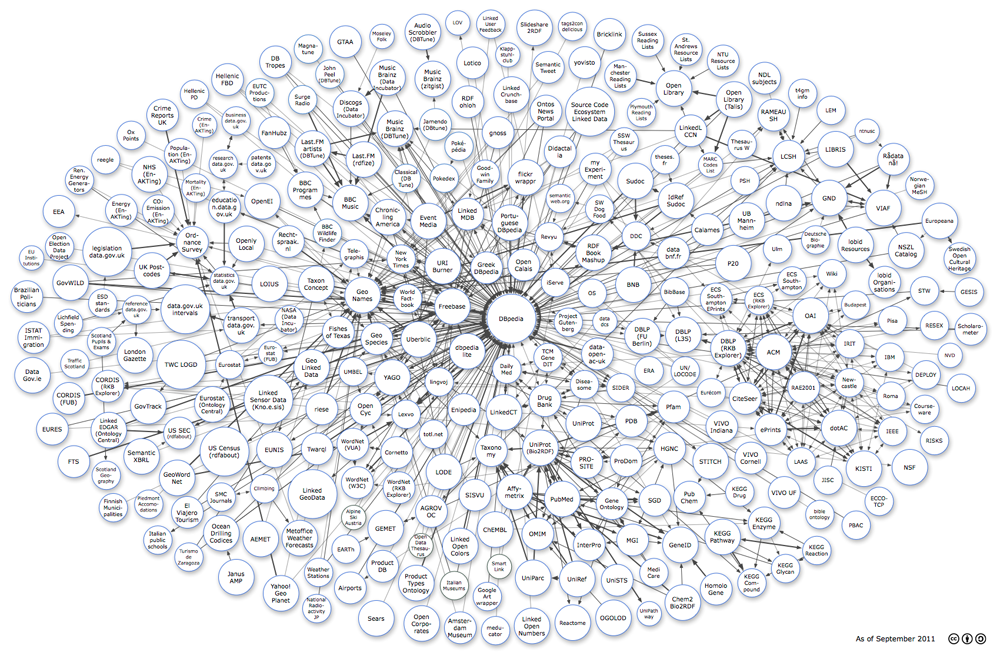
\includegraphics[width=1.0\textwidth]{lod-cloud.png}    
  \caption[The Linked Open Data cloud as of September 2010.]{The Linked Open Data cloud as of September 2010, by Richard Cyganiak and Anja Jentzsch. Source: \url{http://lod-cloud.net/}}    
  \label{fig:lod-cloud}
  \end{center}  
\end{figure}

\section{Conclusion}
In this chapter, we have first introduced the Semantic Web,
and compared it to the non-semantic Web.
We have shown how structured data in form of tables
is a~first step towards richer semantics.
An example of converting structured data from Wikipedia
to machine-readable data is the knowledge base DBpedia.
Further, we have looked at the intrinsic semantics of HTML in versions 4 and 5,
and how through additional attributes even richer semantics can be added
by the annotation formats Microformats and Microdata.
We have formally introduced the Resource Description Format (RDF)
and its different serializations.
On top of RDF, we have detailed how the Semantic Web query language SPARQL
can be used to express queries across data sources.
Finally, we have shown how data on the Web can be exposed as so-called Linked Data,
an effort which gets visible in the Linked Open Data cloud.
With these Semantic Web background technologies,
we have set the foundations for the coming chapters that build upon those pillars.